\begin{figure}[h]
    \centering
    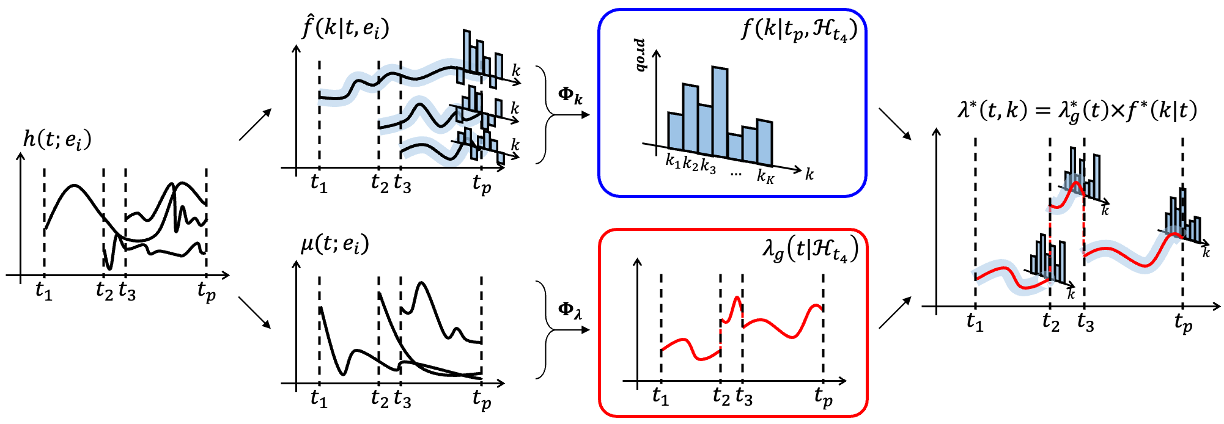
\includegraphics[width=0.95\linewidth]{figure/main_figure_final.png}
    \caption{\small Overview of the proposed framework. Hidden states corresponding to each event $e_i$ are individually propagated and decoded into trajectories $\mu(t;e_i)$ and $\hat{f}_k (k|t, e_i)$. These trajectories represent the influence of individual events on the MTPP, which is reconstructed by aggregating all the trajectories.}
    \label{fig:main}
\end{figure}

\section{Decoupling Marked Temporal Point Processes}
This work introduces a generalizable framework designed to effectively model MTPP distributions through decoupled structures. 
For a sequence of events $\mathcal{S} = \{e_i\}_{i=0} ^n$, where each event $e_i = (t_i, k_i)$ consists of a timestamp $t_i$ and a marker $k_i$, the objective is to predict the distribution of the next event $e_{n+1}$. 
Rather than directly estimating the conditional intensity $\lambda^*(t,k)$ as in prior approaches, we adopt a decoupled modeling strategy by separately estimating the ground intensity $\lambda^*_g(t)$ and the event distribution $f^*(k|t)$.

In our framework, the temporal influence of each event is captured by hidden state dynamics $h(t;e_i)$, which are decoded to yield $\lambda^*_g(t)$ and $f^*(k|t)$. As shown in Fig.~\ref{fig:main}, these two components are modeled as separate trajectories and are combined to recover $\lambda^*(t,k)$.

\subsection{Hidden State Dynamics \label{continuous modeling}}

The framework incorporates hidden state dynamics that are decoupled for each event. These hidden states characterize the impact of an event $e_i$ on the overall process.
The decoupled hidden states, $h(t; e_i) \in \mathbb{R}^d$ for $i = 1, \cdots, n$, evolve independently over time from the occurrence of each event at $t_i$. These dynamics are parameterized using Neural ODEs~\cite{bib:node} to model the intricate behavior of the intensity function in MTPP.

The initial state $h(t_i;e_i)$ depends on the event type $k_i$, and the dynamics are computed by solving an initial value problem (IVP). The hidden state for event $e_i$ at time $t$ is given as:
\begin{align}
d h(t;e_i) &=  \gamma(h(t;e_i), t, k_i;\theta) dt, \\
h(t;e_i) &= h(t_i;e_i) + \int_{t_i}^t \gamma(h(s;e_i), s, k_i;\theta) ds \nonumber \\
&= W_{e}(k_i) + \int_{t_i}^t \gamma(h(s;e_i), s, k_i;\theta) ds,
\label{eq:hiddenS}
\end{align}
where $W_e(\cdot): \{1, \cdots, K\} \rightarrow \mathbb{R}^d$ is a trainable embedding, and $\gamma$ is a neural network parameterized by $\theta$. Since $h(t;e_i)$ is decoupled, hidden states at time $t$ can be computed in parallel as a multidimensional ODE:
\begin{align}
    \frac{d}{dt} \mathbf{h}(t) = 
    \frac{d}{dt}
    \begin{bmatrix}
        h(t;e_0) \\
        \vdots \\ 
        h(t;e_i)
    \end{bmatrix}
    = 
    \begin{bmatrix}
        \gamma(h(t;e_0), t, k_0;\theta) \\ 
        \vdots \\ 
        \gamma(h(t;e_i), t, k_i;\theta)
    \end{bmatrix}.
    \label{eq:hidden_parallel}
\end{align}

The decoupled structure enables selective use of hidden states when computing $f^*(t)$ under specific histories $\mathcal{H}_t$, such as omitting $h(t;e_{j+1})$ when $t > t_{j+1}$. Detailed usage is described in Sec.~\ref{sec:ground int}.

\subsection{Ground Intensity Function \label{sec:ground int}}

The ground intensity $\lambda^*_g(t)$ is modeled as a combination of event-specific \textit{influence functions} $\mu(t;e_i)$, which generalize the excitation functions in Hawkes processes~\cite{bib:hawkes}. To compute $\lambda_g(t|\mathcal{H}_t)$, the influences of historical events are aggregated:
\begin{align}
    \lambda_g(t|\mathcal{H}_{t_{n+1}}) = \Phi_\lambda(\mu(t;e_0), \cdots, \mu(t;e_n)),
    \label{eq:lambdag}
\end{align}
where $\mu(t;e_i) := g_\mu(h(t;e_i))$, decoded via a neural network $g_\mu: \mathbb{R}^d \rightarrow \mathbb{R}$. The aggregation function $\Phi_\lambda$ ensures non-negativity. Decoding $\mu(t;e_i)$ prior to aggregation ensures visibility of individual event influences.

\subsection{Integration and Prediction via Neural ODEs}

The computation of various quantities such as likelihood, survival rates, and expected values in MTPP necessitates integration. Neural ODEs, being computationally demanding due to sequential solvers, are leveraged efficiently by solving multi-dimensional differential equations:
\begin{align}
\label{eqn:multi-integral}
{\partial \over \partial t} 
\begin{bmatrix}
\mathbf{h}(t) \\[1.5ex] 
\Lambda_g (t |  \mathcal{H}_{t_i}) \\[1.5ex] 
F(t | \mathcal{H}_{t_i}) \\[1.5ex] 
\mathbb{E}[t]
\end{bmatrix}
= 
\begin{bmatrix}
\gamma (\mathbf{h}(t),t, \mathbf{k}; \theta) \\[1.5ex] 
\lambda_g(t | \mathcal{H}_{t_i}) \\[1.5ex] 
f(t|\mathcal{H}_{t_i}) \\[1.5ex] 
t \cdot f(t|\mathcal{H}_{t_i})
\end{bmatrix}
= 
\begin{bmatrix}
\gamma (\mathbf{h}(t),t,\mathbf{k}; \theta) \\[1.5ex] 
\Phi_\lambda( g_\mu(\mathbf{h}(t))) \\[1.5ex] 
\lambda_g(t|\mathcal{H}_{t_i}) \cdot \exp (\Lambda_g(t_{i-1}|\mathcal{H}_{t_i}) - \Lambda_g(t|\mathcal{H}_{t_i}) ) \\[1.5ex] 
t \cdot f(t|\mathcal{H}_{t_i}) 
\end{bmatrix}
\end{align}

This eliminates the need for separate integration steps, enabling simultaneous computation of multiple quantities, as visualized in Fig.~\ref{fig: selective DE}.
Therefore, important estimations with integration, such as likelihood, survivor rate $S ^* (t) := 1- F^*(t)$, and $\mathbb{E}_{f^*} [t]$ can be predicted in a single run. 
This formulation can be applied to any number of integrations.

\begin{wrapfigure}{r}{0.44\textwidth}
    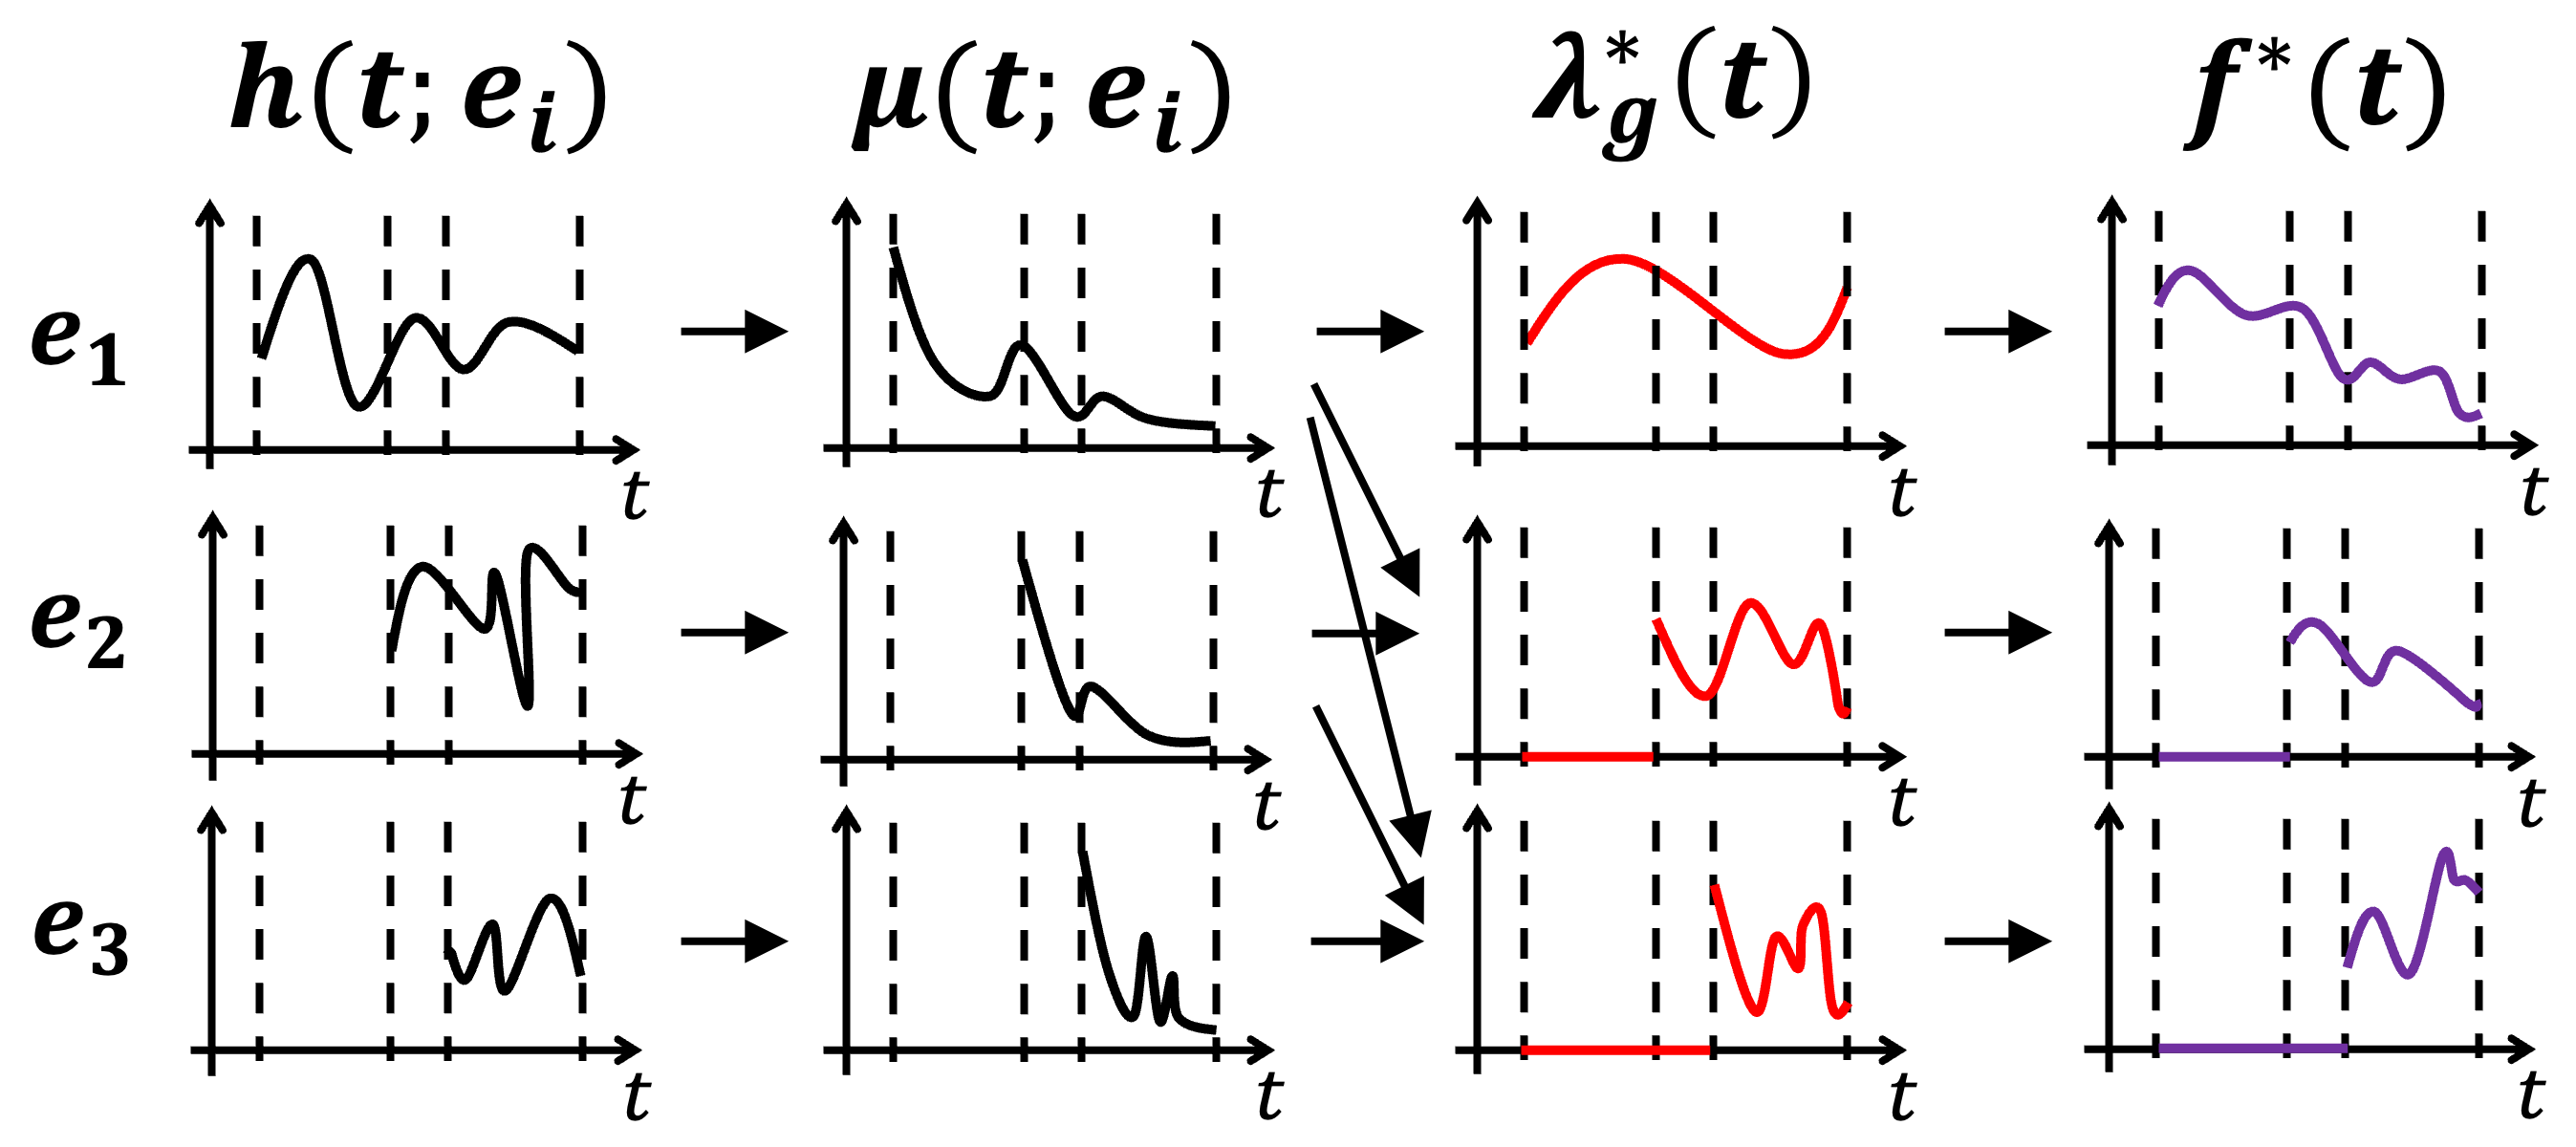
\includegraphics[width=0.42\textwidth]{figure/eq_9_figure2.png}
    \captionsetup[figure]{font=small}
    \caption{\small Visualization of \eqref{eqn:multi-integral}. Different combinations of $\mu(t;e_i)$ can be selected for calculating $\lambda ^*_g(t)$ and $f^*(t)$ conditioned on different $\mathcal{H}_{t_i}$ in parallel.}
    \label{fig: selective DE}
\end{wrapfigure} 
Moreover, as briefly mentioned in Sec. \ref{continuous modeling}, the influence functions can be selected according to our interests as illustrated in Fig. \ref{fig: selective DE}. 
Therefore, approximations of functions in \eqref{eqn:multi-integral} under different $\mathcal{H}_{t_i}$ can be obtained in parallel, distinguishing Dec-ODE from other intensity-based methods that require separate runs. 


\subsection{Conditional Probability for Marks \label{sec:fk}}

The conditional probability of marks $f^*(k|t)$ is formulated as:
\begin{equation}
 f(k|t, \mathcal{H}_{t_{n+1}}) = \Phi_k(\hat{f}(k|t,e_0), \cdots, \hat{f}(k|t,e_n)),
\end{equation}
where $\hat{f}(k|t,e_i):= g_f(h(t;e_i))$ and $\Phi_k$ ensures $\sum_K \Phi_k(\cdot) = 1$. This approach captures temporal dynamics in the event context, such as changing probabilities over time.

\section{Linear Dec-ODE}
\subsection{Combining Influences from Past Events}
To demonstrate the proposed framework's effectiveness, we implement a linear variant of Dec-ODE. Here, $\Phi_\lambda$ and $\Phi_k$ are defined as simple linear combinations while satisfying the constraints using activation functions:
\begin{align}
\lambda_g(t|\mathcal{H}_{t_{n+1}}) &= \sum_{e_i \in \mathcal{H}_{t_{n+1}}} \text{softplus}(\mu(t;e_i)), \label{eq: lin-ground}\\
f(k|t, \mathcal{H}_{t_{n+1}}) &= \text{softmax}\left(\sum_{e_i \in \mathcal{H}_{t_{n+1}}} \hat{f}(k|t,e_i)\right).
\end{align}

The linearity offers interpretability and scalability while supporting complex temporal dynamics beyond classical Hawkes processes. 

\subsection{Training Objective \label{sec:obj}}

The goal of our approach is to maximize the likelihood of the predicted Marked TPP \cite{bib:daley}. Taking the logarithm of the likelihood in \eqref{eq:likelihood}, we obtain:
\begin{equation}
\begin{aligned}
\ln f(t, k) &= \ln \bigg[\prod^{\mathcal{N}_g(t_N)}_{i=1} \lambda^*_g(t_i)\bigg] \bigg[\prod^{\mathcal{N}_g(t_N)}_{i=1} f^*(k_i | t_i) \bigg] \exp\bigg(- \int_0^{t_N} \lambda^*_g(u) du \bigg) \\
 &= \underbrace{\sum^{\mathcal{N}_g(t_N)}_{i=1} \ln \lambda^*_g(t_i) - \int_0^{t_N} \lambda^*_g(u) du}_{\ln L_\lambda} + \underbrace{\sum^{\mathcal{N}_g(t_N)}_{i=1} \ln f^*(k_i | t_i)}_{\ln L_k},
\label{eq:obj}
\end{aligned}
\end{equation}
where $t_N$ is the final observed time point. The log-likelihood terms $\ln L_\lambda$ for the ground intensity and $\ln L_k$ for the mark distribution are defined separately and are used to learn $\lambda_g(t)$ and $f(k | t)$, respectively.

Conceptually, the first term in $L_\lambda$ captures the likelihood of events occurring at each $t_i$, while the second term accounts for the likelihood of events not occurring at all other times. To maximize $L_\lambda$, $\lambda^*_g(t)$ should be high at event occurrence times and low otherwise. 
Additionally, for estimation purposes, $f(t)$ is normalized to satisfy $\int f(t) dt = 1$.

\subsection{Training Scheme \label{train_parallel}}
% \vspace{-5pt}
Prior works leveraging differential equation-based modeling \cite{bib:NJSDE, bib:STPP} typically solve over the entire time range sequentially, resulting in substantial training time. In contrast, our approach mitigates this limitation by utilizing the properties of $\Phi_\lambda$ with linear summation, as described below.

First, since each $\mu(t; e_i)$ evolves independently of other events, they can be propagated simultaneously by solving a multi-dimensional differential equation:
\begin{equation}
    d 
    \begin{bmatrix}
        \mu(\tau_0 ;e_0) \\ \vdots \\ \mu(\tau_i;e_i)
    \end{bmatrix}
    = 
    \begin{bmatrix}
        \gamma(\mu(\tau_0), \tau_0, k_0;\theta) \\ \vdots \\ \gamma(\mu(\tau_i), \tau_i, k_i; \theta)
    \end{bmatrix}
    \cdot d \boldsymbol{\tau},
    \label{eq: train_parallel}
\end{equation}
where $ \boldsymbol{\tau} =[\tau_0, \cdots, \tau_i]^\top = [t_0 + t, t_1 + t, \cdots, t_i + t]^\top$. 

Second, formulating the ground intensity as a linear equation offers the advantage of computing the compensator $\Lambda^*_g(t)$ in a similar manner to \eqref{eq: lin-ground}:
\begin{align}
    \Lambda^*_g(t) & = \int_0^t \lambda_g^*(s) ds = \int_0^t \sum_{e_i \in \mathcal{H}_{t}} \text{softplus}(\mu(s; e_i)) ds \\    
    & = \sum_{e_i \in \mathcal{H}_{t}} \int_{t_i}^t \text{softplus}(\mu(s; e_i)) ds,
    \label{eq:Lambda}
\end{align}
where the integration bounds shift because the influence of $e_i$ begins only after $t_i$. 

Equation \eqref{eq:Lambda} illustrates that the integration in \eqref{eq:obj} can be performed by independently integrating $\text{softplus}(\mu(t; e_i))$ for each event and subsequently summing the results, rather than sequentially processing the entire sequence. Consequently, given a fixed number of time points $m$, the full trajectory can be solved in a fixed number of steps. The efficiency of this approach is further discussed in Sec. \ref{ablation: parallel}.
